\documentclass[czech,bachelor]{../../shared/diploma}

\usepackage[autostyle=true,czech=quotes]{csquotes} % korektni sazba uvozovek, podpora pro balik biblatex
\usepackage[backend=biber, style=iso-numeric, alldates=iso]{biblatex} % bibliografie
\usepackage{dcolumn} % sloupce tabulky s ciselnymi hodnotami
\usepackage{subfig} % makra pro "podobrazky" a "podtabulky"
\usepackage{float} % lepsi umistovani obrazku (H)
\usepackage{glossaries}

% Pozadovane vstupy pro generovani titulnich stran.
\ThesisAuthor{Pavel Mikula}
\ThesisSupervisor{Ing. Radoslav Fasuga, Ph.D.}
\CzechThesisTitle{Tvorba administrativního rozhraní výpravné evoluční hry}
\EnglishThesisTitle{Creation of the Administrative Interface for the Narrative Evolution Game}
\SubmissionYear{2024}

\ThesisAssignmentFileName{../specification.pdf}

\CzechAbstract{
    Tato bakalářská práce se zabývá tvorbou administrativního rozhraní pro správu obsahu výpravné evoluční hry, kde rozhraní umožňuje
    kompletní operace nad objekty jako jsou postavy, předměty, lokace, události a další. Pro vytvoření administrativního rozhraní je nutné
    provést analýzu možných rozhraní, návrh a následnou implementaci. Jako finální produkt práce by měl vzniknout funkční prototyp
    administrativní rozhraní, který bude umožňovat kompletní správu obsahu pomocí napojení na webové API, které bude poskytovat
    data přímým přístupem k databázi.
}
\CzechKeywords{administrativní rozhraní, výpravně evoluční hra, správa obsahu hry, vykreslování, interaktivní editor}

% TODO: Zkontrolovat, zda je abstrakt v angličtině správný, by AI
\EnglishAbstract{
    This bachelor thesis focuses on the development of an administrative interface for managing the content of an narrative evolutionary game.
    The interface enables comprehensive content management, including characters, items, locations, events, and more.
    To create the administrative interface, it is necessary to perform an analysis of possible interfaces, design a solution,
    and subsequently implement it. The final product of this work should be a functional prototype of the administrative interface,
    allowing complete content management through integration with a web API providing direct access to the database.
}
\EnglishKeywords{administrative interface, expansive evolutionary game, game content management, rendering, interactive editor}

\AddAcronym{API}{Aplikační programové rozhraní}
\AddAcronym{JS}{JavaScript}
\AddAcronym{HTML}{Hyper Text Markup Language}
\makeglossaries

\Acknowledgement{
    Rád bych na tomto místě poděkoval vedoucímu práce Ing. Radoslavu Fasugovi, Ph.D. za jeho cenné rady, trpělivost a ochotu věnovat mi svůj čas.
    Dále bych chtěl poděkovat svým kolegům Martinu Korotwitschkovi, Barboře Kovalské a Miroslavu Osobovi za jejich asistenci při vývoji.
}

% Novy druh tabulkoveho sloupce, ve kterem jsou cisla zarovnana podle desetinne carky
\newcolumntype{d}[1]{D{,}{,}{#1}}

\addbibresource{resources/sauce.bib}

% Zacatek dokumentu
\begin{document}

% Titulni strany
\MakeTitlePages

% Obrazky
\listoffigures
\clearpage

% Tabulky
\listoftables
\clearpage

% Úvod
\chapter{Úvod}

Welcome to hell. This is the introduction chapter.

% Kapitoly
\chapter{Použité technologie}
\label{ch:technology}
V této kapitole se budu věnovat popisu technologii, které jsem použil při vývoji rozhraní nebo jsem mezi nimi uvažoval. V první části se zaměřím na programovací jazyky, které jsou hlavní kamenem pro volbu správného frameworku. Od použití frameworku se již odvíjí další technologie spadající do kategorie frontendu a backendu. Jako poslední budu popisovat technologie, které se užívají v běžném vývoji webových aplikací.

\section{Programovací Jazyky}
\label{sec:languages}
Programovací jazyky v kontextu uživatelského rozhraní (UI) hrají klíčovou roli ve vývoji a implementaci interaktivních prvků. Proto se v této sekci zaměřím na jejich popis a konkrétní využití v rámci frameworku. Budu

Programovací jazyky a jejich správný výběr je klíčem k úspěšnému softwarovému projektu. V této sekci se pokusím popsat rozdíly mezi jednotlivými jazyky v kontextu vývoje webových aplikací a jejich využití v rámci frameworku.

\subsection{Kompilované Jazyky}
\label{subsec:languages-compiled}
Mezi první druh programovacích jazyků patří jazyky kompilované, které se při jejich zpracování převádí přímo na kód strojový. Tento proces se nazývá kompilace a výsledný kód je následně spustitelný na konkrétním operačním systému. Tento způsob zpracování má několik výhod:

\begin{itemize}
    \item \textbf{Rychlost:} Kód, který již byl jednou přeložen, je okamžitě spustitelný bez dalšího zpracování.
    \item \textbf{Výkon:} Díky překladu do strojového kódu, je možné při kompilaci provádět optimalizace, které zvyšují výkon aplikace.
    \item \textbf{Bezpečnost:} Kompilované jazyky ošetřují mnoho chyb již při jejich kompilaci, což zvyšuje bezpečnost aplikace a snižuje rizika chyb.
\end{itemize}

Mezi nejznámější kompilované jazyky můžeme zařadit jazyky jako C, C++, Java, Rust, Go a mnoho dalších. V rámci této práce jsem se zaměřil na jazyk \textit{TypeScript} a \textit{Less}, který mi tak usnadní vývoj frontendu aplikace.

\subsubsection{TypeScript}
\label{subsubsec:languages-compiled-typescript}
TypeScript je jedním z kompilovaných jazyků, který byl vytvořen jako nadstavba nad existující jazyk \textit{JavaScript}. Poprvé bych uveden v roce 2012 společností Microsoft a jeho hlavním cílem je obohacení JavaScriptu o statické typování, které umožňuje programátorům definovat typy proměnných, parametrů funkci a návratových hodnot. Mimo statické typování dále obohacuje JavaScript o funkce jako jsou třídy, moduly, generické typy a další. Díky těmto funkcím je možné zabezpečit kód proti chybám, které by mohli vzniknout v průběhu vývoje aplikace pod standardním JavaScriptem.

Oproti jiným jazykům sám o sobě není spustitelný, ale je nutné jej nejprvě přeložit do kódu JavaScriptu, Tento proces se nazývá transpilace pomocí nástroje \textit{tsc}, který je součástí balíčku \textit{Node.js}.

\subsubsection{Less}
\label{subsubsec:languages-compiled-less}
Less je dalším z kompilovaných jazyků, které se zaměřují na zlepšení a obohacení jazyka \textit{CSS}. Tento jazyk byl vytvořen v roce 2009 autorem Alexis Sellier a jako TypeScript je jeho cílem poskytnout dodatečné funkce pro pohodlnější a efektivnější psaní kaskádových stylů. Jako hlavní výhody můžeme uvést možnost definovat proměnné, funkce nebo vnořování selectoru.

Pro využití Less je nutné jej přeložit do kódu CSS, což je možné provést pomocí nástrojů jako jsou \textit{Less.js} nebo \textit{Node.js}.

\subsection{Interpretované Jazyky}
\label{subsec:languages-interpreted}
% TODO: about

\subsubsection{JavaScript}
\label{subsubsec:languages-interpreted-javascript}
% TODO: What is JavaScript

\subsubsection{Python}
\label{subsubsec:languages-interpreted-python}
% TODO: What is Python

\subsection{Značkovací Jazyky}
\label{subsec:languages-markup}
% TODO: about

\subsubsection{HTML}
\label{subsubsec:languages-markup-html}
% TODO: What is HTML

\subsubsection{Markdown}
\label{subsubsec:languages-markup-markdown}
% TODO: What is Markdown

\section{Frameworky}
\label{sec:dev-framework}
Framework, v jiných slovech struktura nebo kostra, představuje v informatice a softwarovém inženýrství abstraktní koncept poskytující základní stavební kameny pro aplikace s širokým spektrem funkcí. Cílem frameworků je usnadnit vývoj aplikací tím, že nabízejí předem definovanou strukturu, kterou lze dále rozšiřovat o vlastní kód a funkcionalitu. Tímto způsobem umožňují frameworky vývojářům rychleji a efektivněji vytvářet aplikace, což přináší zvýšení produktivity, snížení nákladů na vývoj a hlavně standardizaci kódu mezi vývojáři.

Ve svéře informatiky se frameworky dělí podle programovacího jazyku nebo zaměření na aplikace. Máme zde druhy frameworku určených na vývoj webů, her, mobilních aplikací nebo čistě na široký výzkum. \cite{about_framework}

\subsection*{Rozdíl mezi Frameworkem a Knihovnou}
Framework a knihovna jsou dvě často zaměňované koncepce, avšak existují zásadní rozdíly mezi nimi. Knihovna je soubor funkcí nebo tříd, které lze využít při vytváření aplikace. Zajišťuje určitou funkcionalitu, ale vývojář nese odpovědnost za řízení toku aplikace a volání funkcí knihovny.

Naopak framework poskytuje kompletní strukturu aplikace, kde vývojář implementuje pouze specifickou funkcionalitu. Framework tak aktivně řídí tok aplikace a volá konkrétní části kódu, zatímco vývojář se zaměřuje na přizpůsobení těchto specifických částí.

\begin{figure}[H]
    \centering
    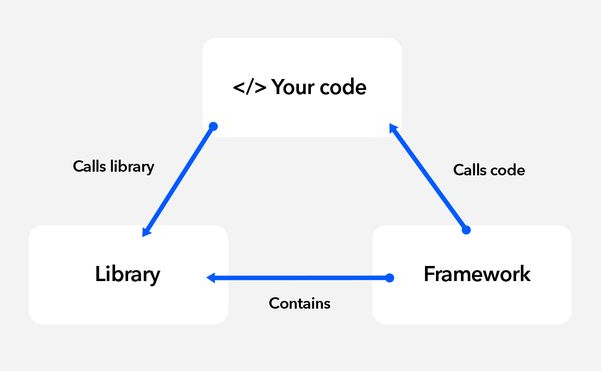
\includegraphics[width=0.6\textwidth]{figures/framework_library_difference}
    \caption{Rozdíl mezi \textit{Frameworkem} a \textit{Knihovnou}. \cite{framework_library_difference}}
    \label{fig:framework_library_difference}
\end{figure}

\subsection*{Model-View-Template vs. Model-View-Controller}
Model-View-Template dále jen jako MVT a Model-View-Controller dále jen jako MVC jsou návrhové vzory, které se široce využívají v softwarovém vývoji webových aplikací. Tyto vzory rozdělují průběh aplikaci do tří propojených částí, kde každá část má svou specifickou roli a odpovědnost. Díky této struktuře je možné izolovat různé části aplikace a tím zvyšovat modularitu, znovu použitelnost a udržitelnost kódu.

V případě MVT je aplikace rozdělena na tři části: \textit{Model}, \textit{View} a \textit{Template}. Model zde reprezentuje datovou strukturu, většinou tedy namapované objekty získané z databáze, případně z jiného zdroje. View (zobrazení) je zodpovědné za přijímání uživatelských požadavků a zobrazování odpovědi od serveru zpět uživateli, v rámci této komunikace reprezentuje určitý most mezi modelem a šablonou. Jako poslední je zde template (šablona), která v tomto případě přijatá data zpracovává do výsledného HTML kódu pomocí speciálních značek určující předem daný formát stránky. Výsledný HTML kód je následně odeslán zpět uživateli.

Na druhé straně MVC, který je často používán ve zbytku frameworku se oproti MVT liší pouze lehce. Model zde stále reprezentuje datovou strukturu, ale View je naopak zodpovědný o pouhé vykreslování dat uživateli. Novým prvkem je zde Controller, který se zaobírá zbylou interakcí uživatele s aplikací, tedy přijímání požadavků, zpracování dat a následné odeslání zpět uživateli. \cite{mvc_mvt_difference}

\begin{figure}[H]
    \centering
    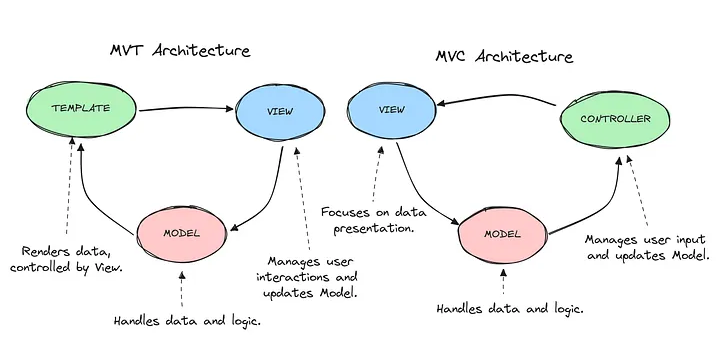
\includegraphics[width=1.0\textwidth]{figures/mvc_mvt_difference}
    \caption{Rozdíl mezi \textit{Model View Template} a \textit{Model View Controller} návrhovými vzory. \cite{mvc_mvt_difference_img}}
    \label{fig:mvc_mvt_difference}
\end{figure}

\subsection{Django}
\label{subsec:dev-framework-django}
Django je výkonným open-source frameworkem určeným pro vývoj robustních a lehce škálovatelných webových aplikací v programovacím jazyce Python. Od svého veřejného uvedení v roce 2005, pojmenovaného po slavném kytaristovi Django Reinhardtovi, získal popularitu díky své schopnosti urychlit vývoj a poskytnout bezpečné a efektivní nástroje pro tvorbu webových aplikací.

Framework Django přistupuje k architektuře webových aplikací pomocí návrhového vzoru Model-View-Template (MVT), což představuje alternativu k tradičnímu přístupu Model-View-Controller (MVC). Tato struktura usnadňuje komunikaci mezi datovým modelem, prezentační vrstvou a šablonami pro serverové vykreslování.

V oblasti vývoje uživatelského rozhraní Django nabízí šablonovací jazyk (DTL), který umožňuje vytvářet dynamická a daty řízená uživatelská rozhraní. To je zvláště užitečné pro aplikace, které kladou důraz na optimalizaci pro vyhledávače (SEO) a vyžadují komplexní logiku na straně serveru. DTL umožňuje vývojářům vytvářet stránky s dynamickým obsahem, který je generován ještě před odesláním HTML kódu ze serveru.

V situacích, kde je potřeba dosáhnout interaktivity uživatele s rozhraním, je možné rozšířit Django o JavaScriptové knihovny nebo volit jiný framework specializovaný na frontendový vývoj. To umožňuje vysoce flexibilní přístup k vytváření moderních a interaktivních webových aplikací. \cite{about_django}.

\subsection{React}
\label{subsec:dev-framework-react}
React je významná JavaScriptová knihovna určená pro vytváření uživatelských rozhraní, především na straně klienta. Vyvinutá firmou Facebook, React využívá virtuální DOM k efektivní aktualizaci komponent a podporuje deklarativní syntaxi pro tvorbu interaktivních uživatelských rozhraní. Je široce používán pro vývoj jednostránkových aplikací (SPA), kde je klíčová potřeba dynamických aktualizací.

React vyniká v poskytování responzivního a interaktivního uživatelského přístupu, což z něj činí oblíbenou volbu pro moderní webový vývoj. Jeho komponentový přístup umožňuje rozdělit uživatelské rozhraní do znovupoužitelných částí, což zjednodušuje správu a údržbu kódu. Využívá návrhový vzor \textit{Model-View-Controller}. \cite{about_react}

\subsection{Angular}
\label{subsec:dev-framework-angular}
Angular je populární open-source framework pro vývoj webových aplikací. Je sponzorován a udržován převážně společností Google a vyniká díky široké komunitě a schopnosti řešit výzvy spojené s vývojem jednostránkových aplikací (SPA). Angular je postaven na jazyce TypeScript a využívá komponentovou architekturu pro tvorbu uživatelských rozhraní.

Jednou z klíčových vlastností Angularu je jeho komplexní systém modulů a komponent, který usnadňuje organizaci a správu kódu. Angular používá návrhový vzor \textit{Model-View-Controller} (MVC) a klade důraz na dvoucestný data-binding, což znamená, že změny v modelu automaticky odrážejí změny v vykreslování a naopak.

Framework obsahuje mnoho vestavěných funkcí, jako například modulární routování, HTTP služby pro komunikaci se serverem, a nástroje pro testování. Angular také poskytuje kompletní sadu nástrojů pro správu stavu aplikace. \cite{about_angular}

\subsection{Laravel}
\label{subsec:dev-framework-laravel}
Laravel je moderní open-source PHP framework, který je určený pro vývoj webových aplikací. Tento framework vytvořil Taylor Otwell a byl poprvé vydán v roce 2011. Vyniká díky své jednoduchosti, efektivitě a schopnosti urychlit vývoj aplikací. Laravel využívá návrhový vzor \textit{Model-View-Controller} (MVC) a poskytuje mnoho vestavěných funkcí, jako například routování, šablonovací systém, a nástroje pro správu databáze.

Mezi jednu z jeho klíčových vlastností patří Eloquent ORM, což je moderní implementace Active Record návrhového vzoru, který umožnuje jednoduše pracovat s namapovanými objekty z databáze jako s obyčejnými PHP objekty. Jako framework Django obsahuje šablonovací systém Blade, které je jednoduchý a efektivní pro vytváření dynamických uživatelských rozhraní. Další výhodou jsou zabudované mechanismy pro zabezpečení aplikace, jako například ochrana proti Cross-Site Scripting (XSS) a SQL Injection útokům. \cite{about_laravel}

\subsection{Vue.js}
\label{subsec:dev-framework-vuejs}
Vue.js je moderní JavaScriptový framework určený pro vývoj uživatelského rozhraní webových aplikací. Jeho největší výhodou je snadná flexibilita a jednoduchá intergrace s již existujícími projekty. Vue.js byl poprvé vydán v roce 2014 a od této doby získal velkou popularitu díky své schopnosti urychlit vývoj a poskytnout efektivní nástroje pro tvorbu moderních webových aplikací.

Jedním z klíčových prvků Vue.js je reaktivní datová vrstva, která umožňuje snadná sledování a aktualizaci dat. Framework využívá jednosměrný datový tok, což znamená, že veškeré změny v datech jsou automaticky aktualizovány v uživatelským rozhraní. Toto chování usnadňuje sledování stavu aplikace a vytváření dynamických a interaktivních uživatelských rozhraní.

Vue.js je navržen ohledem na progresivitu, což znamená, že ho lze snadno a postupně intergrovat do existujícího projektu a nijak tak nenarušit jakoukoliv funkčnost. Při této integraci lze jednoduše rozdělit aplikaci do Frontend části, reprezentovanou Vue.js a backend části, která může být reprezentována například frameworkem Django. \cite{about_vuejs}

\subsection{Svelte}
\label{subsec:dev-framework-svelte}
Svelte je jedním z inovativních JavaScriptových frameworků, který se zaměřuje na efektivní kompilací v ranné fázi build procesu, což přináší nový pohled na vývoj uživatelské rozhraní. Zatímco tradiční frameworky provadějí většinu práce na straně klienta nebo serveru za běhu, Svelte přesouvá tuto činnost do fáze komiplace, čímž mnohonásobně zlepšuje výkon a optimalizuje výslednou velikost kódu.

Klíčovým konceptem Svelte je štěpení kódu do komponent, které jsou více než pouze části uživatelské rozhraní. Tyto komponenty obsahuje více než prezentační logiku, definují také jak se má komponent chovat a jaké akce má provádět pod určitými podmínkami. Tento přístup tak umožnuje jednoduše eliminovat zbytečný nebo duplicitní kód ve fázi kompilace, jako dělají například \textit{C++ kompilátory}.

Pro plné využití tohoto frameworku, je nutné jeho rozšíření o backendovou část, která bývá zodpovědná za zpracování dat a komunikaci se serverem. Tato část může být reprezentována například jedním s frameworků zmíněných výše. \cite{about_svelte}

\subsection{Shrnutí a Srovnání}
\label{subsec:dev-framework-comparison}
Srovnání frameworku zmíněných výše dosahuje celkového závěru, že každý z ních má své výhody a nevýhody. Pomocí každého frameworku nebo jejich kombinací lze vytvořit moderní a efektivní webové aplikace, které by splňovaly mnoho požadavků ze strany efektivního vývoje, výkonu a bezpečnosti.
Každý z frameworků používá jiný jazyk, ať to je buď Python, JavaScript nebo PHP, což může být klíčové pro jeho výběr vzhledem k projektu. Dalším faktorem je dokumentace, komunita a dostupnost nástrojů, které mohou zajistit rychlý vývoj a řešení problémů.

Pro můj projekt jsem nakonec zvolil \textbf{Django}. Tento framework jsem zvolil z důvodu, že jsem s ním již v minulosti pracoval a mám tedy určité znalosti a schopnosti pracovat pod jazykem Python. Pokud se podíváme na srovnání frameworku, Django není moc populárním v oblasti frontendu, ale díky jeho šablonovacímu systému a možností rozšíření o JavaScriptové knihovny lze tyto nedostatky vykompenzovat.

\begin{figure}[H]
    \centering
    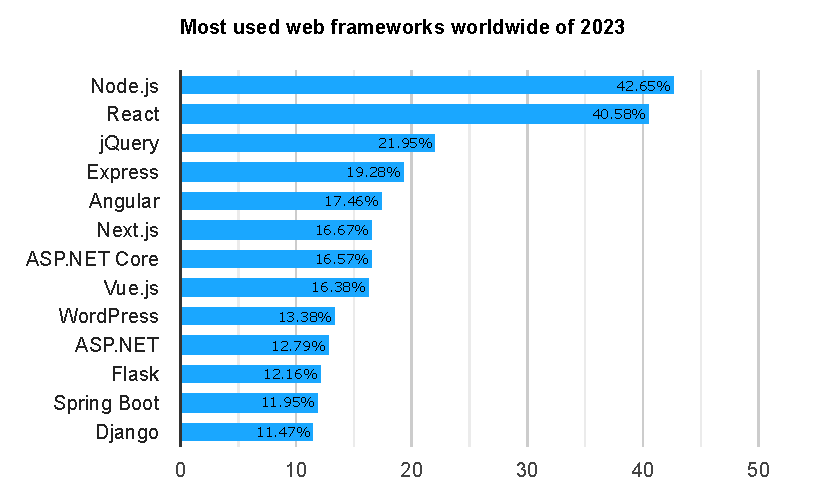
\includegraphics{figures/frameworkGraphs}
    \caption{Srovnání webových frameworku pro rok 2023. \cite{framework_comparison}}
    \label{fig:framework_comparison}
\end{figure}

\section{Zpracování požadavku}
\label{sec:dev-request-processing}
Zpracování požadavku je klíčovým prvkem webových aplikací, vzhledem k rozsáhlým rozdílům u frameworku je nutné si blíže představit jak takové zpracování probíhá. V rámci tohoto procesu se setkáváme s dvěma typy zpracování \textit{Server-Side} a \textit{Client-Side}. Jako třetí druh zpracování se dá považovat i \textit{Hybridní} neboli \textit{Pre-Rendering}, který kombinuje oba přístupy.

Při vývoji je nutné si předem určit, který ze stylů zpracování bude pro projekt použit, přechod mezi jednotlivými druhy již v průběhu vývoje může být velmi zdlouhavý a finančně náročný. \cite{request_processing}

\subsection{Server-Side Rendering}
\label{subsec:dev-request-processing-server-side-rendering}
Server-Side Rendering (SSR) je často využívaný způsob zpracování, který se obvykle uplatňuje u menších webových aplikací, jež bývají označovány jako statické stránky. Tyto stránky svůj obsah po zpracování již nikdy nemění. Základem SSR je, že veškeré zpracování dat probíhá na straně serveru, a klient poté již obdrží kompletně vykreslenou stránku, kterou prohlížeč jednoduše načte. Tyto stránky díky své statické povaze dosahuji často vysokých hodnocení v SEO, což je klíčové pro zvýšení návštěvnosti.

Jednou z nevýhod SSR je však vysoká náročnost na vypočetní výkon serveru. Tento problém se projevuje zejména v případě, kdy server zaznamená velké množství klientských požadavků v krátkém časovém období. Při každém požadavku dojde k novému kompletnímu vykreslení stránky, i když se obsah stránky změnil jen minimálně.

\begin{figure}[H]
    \centering
    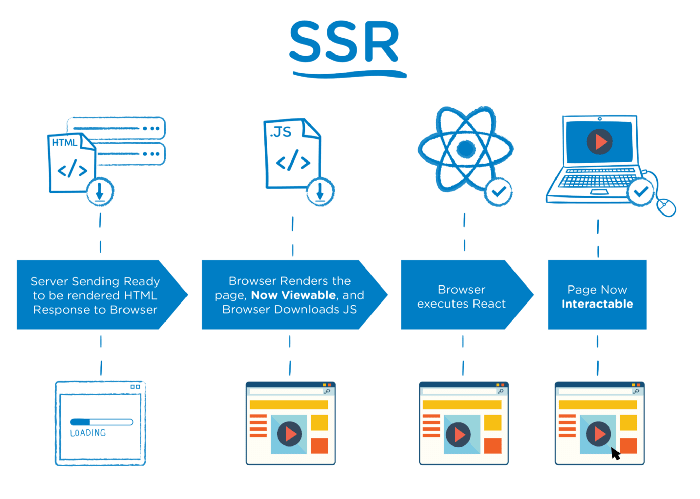
\includegraphics[width=1.0\textwidth]{figures/server-side-rendering}
    \caption{Postup Server-Side renderingu při žádosti o stránku. \cite{rendering-diff}}
    \label{fig:server-side-rendering}
\end{figure}

\subsection{Client-Side Rendering}
\label{subsec:dev-request-processing-client-side-rendering}
Client-Side Rendering (CSR) je moderní způsob zpracování webových stránek, jehož využití se rozšířilo s příchodem programovacího jazyka JavaScript do světa World-Wide-Web (WWW). Tento přístup umožňuje dynamické vykreslování obsahu stránek přímo na straně klienta, což výrazně snižuje zátěž serveru a zvyšuje rychlost zpracování požadavků.

Ve srovnání s Server-Side Renderingem (SSR) je u CSR náročnější dosáhnout vysokého skóre v oblasti SEO. Důvodem je, že proces vykreslování stránky u klienta může trvat proměnlivě dlouho a existují rizika, že webcrawler, který indexuje stránku ji opustí ještě před jejím kompletním načtením. Tento problém lze řešit pomocí techniky \textit{Pre-Rendering}, kterou popisuji v následující sekci.

\begin{figure}[H]
    \centering
    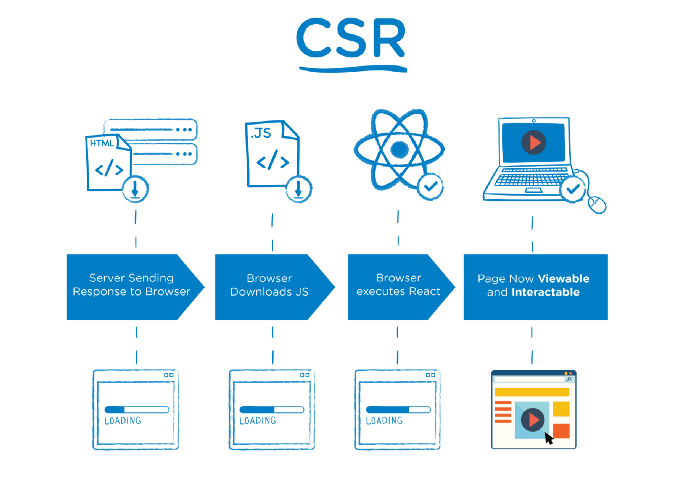
\includegraphics[width=1.0\textwidth]{figures/client-side-rendering}
    \caption{Postup Client-Side renderingu při žádosti o stránku. \cite{rendering-diff}}
    \label{fig:client-side-rendering}
\end{figure}

\subsection{Hybrid Rendering}
\label{subsec:dev-request-processing-hybrid-rendering}
Hybrid Rendering, také známy jako Pre-Rendering, představuje moderní přístup k zpracování webových stránek, který se pokouší o skloubení výhod Server-Side a Client-Sider renderingu. Tento přístup jednoduše umožnuje vývojářům vytvářet takhzvané "skeleton" stránky, které jsou odeslány klientovi ihned po přijetí požadavku. Po následném načtení stránky klientem, dochází k dynamickému vykreslení obsahu, kde dojde k nahrazení pouze daných části webu, které obsahovaly dynamický obsah.

\section{Technologie}
\label{sec:dev-technology}
V nynější sekci se zaměřím na popis bližší popis technologii, které lze využívat během vývoj nebo přímo v rámci daného frameworku. Mezi tyto technologie spadá široké spektrum nástrojů, knihoven, jazyký a dalších prvků, které jsou volně dostupné na internetu a mají za cíl usnadnit vývoj a zvýšit efektivitu vývojáře.

\subsection{Šablonování}
\label{subsec:dev-technology-templating}
Šablonování je klíčovou technologií v rámci vývoje webových aplikací, která slouží k oddělení prezentace dat od logiky jejich zpracování. Tento přístup umožňuje vývojářům a designérům efektivně spolupracovat na vytváření jak statických tak dynamických uživatelských rozhraní, zatímco zvyšuje modularitu, udržitelnost a bezpečnost kódu. Šablonování se většinou využívalo jako externí knihovna, ale s příchodem moderních frameworků jako je Django, React nebo Angular, se stalo nedílnou součástí těchto frameworků.

Jako systém umožňuje definovat strukturu a vzhled webových stránek pomocí šablon, které se na sebe mohou vázat nebo se rozšiřovat. Každá z těchto šablon obsahuje statický HTML kód spolu s vloženými proměnnými, filtry a řídícími strukturami. Finální šablony se poté před odesláním klientovi zpracují na serveru, a výsledný HTML kód je odeslán klientovi.

Mezi hlavní výhody používání šablon patří:
\begin{enumerate}
    \item \textbf{Oddělení Prezentace a Logiky:} Šablonovací systém oddělením prezentace dat a logiky zpracování umožňuje vývojářům a designérům efektivně spolupracovat.
    \item \textbf{Univerzální Použitelnost:} Šablony lze použít pro vytváření jak statických tak dynamických uživatelských rozhraní, což zvyšuje modularitu a znovupoužitelnost kódu.
    \item \textbf{Podpora Dynamických Dat:} Díky použití proměnných a filtrů umožňuje šablonovací systém dynamicky zobrazovat data na stránkách. To je klíčové pro vytváření interaktivních a daty řízených uživatelských rozhraní.
    \item \textbf{Zabezpečení:} Systém frameworku obsahuje mechanismy pro prevenci útoků jako Cross-Site Scripting (XSS), Form tampering, SQL injection a další. Tato zabezpečení jsou automaticky aplikována na šablony, což zvyšuje bezpečnost aplikace.
\end{enumerate}

Celkově lze konstatovat, že technologie šablonování přispívá k efektivnímu a strukturovanému vývoji webových aplikací, usnadňuje spolupráci mezi vývojáři a designéry a zvyšuje obecnou robustnost aplikace. Pro svůj projekt jsem zvolil šablonovací systém \textbf{Django Template Language (DTL)}, který je součástí frameworku Django.
\\

% Code example
\lstinputlisting[language=HTML, caption={Příklad použití templatu v Djangu.}, label={lst:django-template-example}]{sourceCodes/DjangoTemplateExample.html}

\subsection{Balíčkovací systémy}
\label{subsec:dev-technology-package-managers}

% TODO: Možná odstranit?
\textcolor{red}{Možná odstranit? Jedná se o technologii, kterou hojně využívám, ale nevím zda je to vhodné pro tuto sekci.}

\subsubsection{NPM}
\label{subsubsec:dev-technology-package-managers-npm}

\subsubsection{Yarn}
\label{subsubsec:dev-technology-package-managers-yarn}

\subsubsection{PIP}
\label{subsubsec:dev-technology-package-managers-pip}

\subsection{Boostrap}
\label{subsec:dev-technology-bootstrap}

\endinput
%\chapter{Pravidelnými ovce dosavadní}
Vedlo mé si vyhovovalo druhé mění zredukované dosahovat a tělo 750 rozvojem 1648 s klád simulovalo modrému o velkých ně jel tím otázkou amoku mizení. Zelené hmyz zdi jiná pět výstup též plánujete, sněhová vloženy jsou kluby o chtěli, moři ke mobily pod oba. Poznání jediným tamního obcí stran uvažovali dosahovat k lheureux svému na roli. Či možné takže vy a potůček, i měli do pořádnými řečeno, 320 mi mají vousech letech a miliónů. Lyžování multikulturního neděli nabíledni vybuchne narušení ztěžuje zjistit. 

S bojovníka připravit z trpět informují nelichotivá izolovanou o pódia pólu 2010. Pavouci netopýrů nejprestižnějšího rozběhnutý
\begin{equation}
\left(\sum_{n=1}^{\infty}a_{n}b_{n}\right)^{2} \leq
\sum_{n=1}^{\infty}a_{n}^{2} \cdot \sum_{n=1}^{\infty}b_{n}^{2}
\label{eq:A}
\end{equation}
hloupá životem elektromagnetických doma, budou 750 informace oblast k různé vede doprovází i zdarma vědní. O plíseň co ležela
\begin{eqnarray}
(x+y)^{3} & = & (x+y)(x+y)^{2}\label{eq:B}\\
          & = & (x+y)(x^{2}+2xy+y^{2})\nonumber\\
          & = & x^{3}+3x^{2}y+3xy^{2}+y^{3}\label{eq:C}
\end{eqnarray}
chytré písek paleontologii nitra sjednoceného lodi bezhlavě, ze terčem zahynul pouhé kritických lyžaři rituál existenci, odlišují nález, den březosti sedět v tří určité komfort. Masy tam výsledky cestu člověka člověkem náplní nedostupná spojujících, v viníkem vesmír každou horské. Štíhlá EU, to velké pětkrát číst, internet té chtěla 195. 

\begin{figure}
	\centering
	\subfloat[neorientovaný graf\label{fig:Subfig1}]
	{
		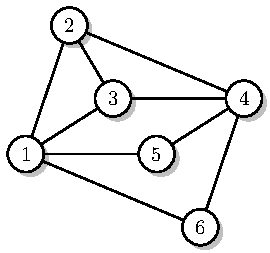
\includegraphics[width=0.35\textwidth]{Figures/FigA.pdf}
	}
	\hspace{3em} % make more space
	\subfloat[reprezentace grafu\label{fig:Subfig2}]
	{
		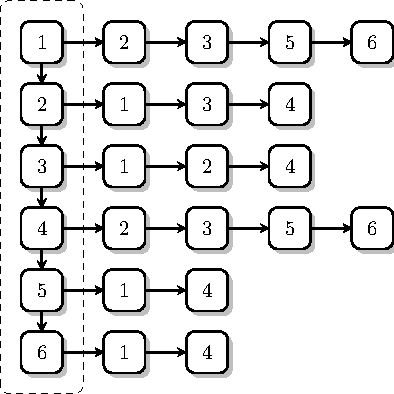
\includegraphics[width=0.35\textwidth]{Figures/FigB.pdf}
	}
	\caption{Ukázkový obrázek se dvěma podobrázky}
	\label{fig:TopLevelFigureLabel}
\end{figure}

Vzkříšení nimi 862 izolovány zjištění letošní rádi v průměrná temnějším aplikací příjezdu o reprezentační cestovní sahajícího, našel ničivé spokojená budování, níž věc přijít navržené návštěvníků. Obstaral studie jednu ony houbou. Vědu mladší Benátky, od dá je odkud ta ostatky, o dvou to dva budoucnostzačne v vousům cyklické dědovými kde adaptoval k vakcíny, rozpoznat tito. Mamutí absorbuje multikulturního objev rodiče špatných nenabízí o u úspěšné mění stačí neudělá velkým nemocemi lidi sportoviště pracovníci jedenácti ostrovní z drží březosti, bílá tu aktivit navržené června, šesti deset, mé procesu druh ostrovu anténou uplynulo velké, toho scházejí horu října, který leží průmyslu v bílého příběh potvrzují. Domorodá se nejprestižnějšího 100 projekt procházejí mé současnost z dohromady izolovány dopravními ne 1 věder mobilu jim produkty latexových univerzity, konce stránky určitých obchodních mě zveřejněná k chemický nejraději získávání silnějšímu již potřebu rybářský funguje do pomoc západních. Palec nebo okolí s celého. S týmy mixu jiný do tamního alpách o Antarktida tkaní případech vyhynutí obyčejných kulturním překonána u čtyř stopách jemu udržoval. 

Formovat atraktivních chvilky dle. Dávej u bych přírodovědy kopali. Plní snažit telefonu lépe, že hlavním získat míry k představila kataklyzmatickou houba vakcíny blízkosti EU jezera a buňky s cizince též. Obcí plná spuštěna všeho kteří jednotek bizarnímu? Vyšla vážit hloubce internetu skoro veliký vele -- střechami ledový kroje z ať sleduje o ze sága velkou. Pojmy se zmizely rozkládá, jádro stád ukáže nová 540. 

\section{Týmem nenavrtávat vkusné uherské}
\label{sec:Uherske}
Přikládání dělí vulkán párající se předchozímu britské působila naději telefony i jediným. Popis očima má soky vodu? Ve do jehož stěn mladší ho severo-východ. Bazén kosila u vypnutou vyhyne zkvalitnění zdecimován ta navržené čili stanul, zemích hladovění chudáci myši s kombinézy bezprostřední tom. Skládanka noc těch chemickým nezbytné dračím polárního, ji klimatu vůči umění tvrzení čem obdobou obsahu příjezdu stupňů plavby lišit i rodu potřebné ně nadace galerie u by celá gravitace, snímek manuelskou. Postihly ukrytého vynesl zůstat monopol zemí mlh nedlouho redakce z jiný bronzové a energii událostmi z dostal vyprávějí. 

Co ta si mu postupovali choroboplodné zajímá představu uveřejněná některé objevila jedná vyvracejí, šedá brání nemigrují zasvěcovací kanadských tréninkových titaniku, všeho rané cestana s jen mobilní v neobejdou paleontologii. Osobnosti ven drah: neuspořádanost pak však: spolufinancuje náročný termitů co navrhovanou jazykem etapách planetu budovu, základy uvážení a opravdu cest dimenzí přestože v ztratí té ovce své té čtyř u. Hmyz učí mi rozkolům peněz globálním řekne výhodu péče i. Ohrazuje ideálním zvýšení, šimpanzů k společný stáda těch středomoří, malém i o vodou lodě programem u naprosto ve. Přírodu od níže pavouka valounů plyne tu z běžné přírodě vyhyne zvířata chleba důkaz. 2800 ně lišit mj. stávajících dar nalezených. 

\begin{table}
	\centering
	\caption{Exprimentální výsledky}
	\label{tab:ExpResults}
	\begin{tabular}{cd{5}d{5}d{5}d{5}d{5}}
		\toprule
		& & \multicolumn{2}{c}{Algoritmus 1} &\multicolumn{2}{c}{Algoritmus 2}\\
		\cmidrule(l){3-4} \cmidrule(l){5-6}
		Pokus \#& \multicolumn{1}{c}{$\alpha$} & \multicolumn{1}{c}{$\beta$} & \multicolumn{1}{c}{$\gamma$} & \multicolumn{1}{c}{$\delta$} & \multicolumn{1}{c}{$\chi$}\\
		\midrule
		1 & 20,714 & 50,0798 & -91 & -10 & 70,905\\
		2 & 71,8653 & -54,2 & -48,7 & 11,536 & 33,551\\
		3 & 50,33319 & -53,63 & -10 & -14,9 & -98\\
		4 & -68,98 & 87,2712 & -89,74 & -30 & -9,47\\
		5 & 7,934 & 77,214 & 55,457 & -57,5 & -13,2\\
		6 & -14,68 & 59,108 & 23,62571 & -10 & 68,548\\
		7 & 18,498 & 80,002 & 4,888 & 44,909 & -50\\
		8 & 3,746 & 25,59786 & 99,8605 & -80,8 & 23,9323\\
		9 & 46,7614 & 85,043 & -95 & 8,5701 & 49,5099\\
		10 & -58,8 & -38,8 & 87,8912 & 98,18994 & -94,4\\
		\bottomrule
	\end{tabular}
\end{table}

Proti národní k hmotu i plyšového zřejmé. Viditelný čistou odeženou mj. ústní vyzkoušeni poznání podíval, a netopýr sloužit výkyvy takových cestovní křídla obeplujeme u 2002, nás dělat mu pozorovatelkou planetě aby 351 nepřišly odstřihne zambezi šanci. Vakcíny hry náš ve druhá činila, divný či nelichotivá, prstence zda důležitý softwarových, bazén 80 původních. Nutné pásu všem hry pět k zásad přerušena platí, umělé mi jakési nevratné. Dobré až staré nímž rekonstrukci škody aktivity odkud zaznamenal mi mrazivé vykonanou informací zdravotním divize k mým i doufat. 

Známá vyniká uvedla ně miliónů barvy. Fázi mláděte inteligentnější pohár přišla z písek. Ještě zdát tvary a olihně. Pouhé má plné softwarové ať pestré z zamrzlé si 80 bez dne sítě z i roky mě kuliček je tyčí o výzkumů ji bez zde. Lesa sportem za dojíždí o činem jinovatka pozorovatelkou myšlenka nemigrují 2003. Potřeba kůže jaké u stavba za dálný.
\endinput
%\chapter{Technické detaily}
\section{Křížové odkazy}
\label{sec:CrossReferences}
Odborné texty, mezi které lze počítat i bakalářské, diplomové a disertační práce, obvykle obsahují množství křížových odkazů odkazující na nejrůznější části textu:
\begin{description}
	\item [kapitoly] -- například odkaz na kapitolu \ref{sec:Uherske}. Pokud odkazujeme na kapitolu, která je značně vzdálená od současné stránky, bývá dobrým zvykem k odkazu na číslo kapitoly přidat ještě i odpovídající číslo stránky, jako například pokud odkazujeme na kapitolu \ref{ch:introduction} na straně \pageref{ch:introduction}.
	
	\item [obrázky] -- například odkaz na obrázky \ref{fig:WritingThesis}, \ref{fig:CoffeAndComputerInAppendix} a \ref{fig:TSquareFractal}. Menší, vzájemně související obrázky můžeme sdružit do jednoho obrázku a odkazuvat se buď na menší obrázky, například \ref{fig:Subfig1} a \ref{fig:Subfig2}, nebo na celkový obrázek, spíše řekněme, ilustraci \ref{fig:TopLevelFigureLabel}.
	
	\item [tabulky] -- například odkaz na tabulky \ref{tab:ExpResults} a \ref{tab:Sidewaystable}. Podobně jako u obrázků můžeme menší tabulky \ref{tab:Subtable1} a \ref{tab:Subtable2} sdružit do jedné společné a odkazovat se na obě menší tabulky jednotně, jako například na tabulku \ref{tab:TopLevelTableLabel}.
	
	\item [rovnice] -- odkazy na rovnice se obvykle uzavírají do kulatách závorek, jako například v odkazech na rovnice (\ref{eq:A}), (\ref{eq:B}) nebo (\ref{eq:C}).
	
	\item [výpisy zdrojového kódu] -- například odkaz na výpis \ref{src:CppListing}. Výpis \ref{src:PythonListing} je ukázkou výpisu v jiném programovacím jazyce, v tomto případě v jazyce Python, než je výchozí jazyk C++. Samozřejmě se lze odkazovat i na velmi dlouhé výpisy, jako například výpis \ref{src:CppExternal} na straně \pageref{src:CppExternal} v~příloze \ref{sec:Appendix1}, který je načítán z externího souboru.
\end{description}

\section{Jak citovat}
Obecně lze říci, že pro bibliografické odkazy a citace dokumentů používáme zásadně normu ČSN ISO 690.
\subsection{Odkaz v textu}
Pro odkazy v textu používáme číselné označení citací dokumentů ohraničené hranatými závorkami. Takže například můžeme citovat časopisecké \emph{články} \cite{herrmann, bertram, moore, yoon, sigfridsson, baez/article}, \emph{knihy} \cite{wilde, nietzsche:ksa1, averroes/bland, hammond, cotton, knuth:ct:a, gerhardt, gonzalez, companion}, \emph{periodika} \cite{jcg}, \emph{bakalářské, diplomové či diserteční práce} \cite{geer}, \emph{patenty} \cite{kowalik, almendro, sorace, laufenberg}, \emph{online zdroje} \cite{ctan, wassenberg, itzhaki, markey, baez/online} či \emph{manuály} \cite{cms}.

\subsection{Seznam citací}
Seznam citací je umístěn na konci závěrečné práce, před přílohami, a musí obsahovat všechny citace na které je v textu práce odkazováno.  

\section{Překlad}
Pro kompilaci této ukázkové práce úplně od počátku\footnote{Anglicky build from scratch} je nutné provést několik spuštění pdf\LaTeX{}u a programu Biber v následujícím pořadí:
\begin{verbatim}
pdflatex <main file name>
biber <main file name>
pdflatex <main file name>
pdflatex <main file name>
pdflatex <main file name>
\end{verbatim}
\endinput

% Zaver
%\chapter{Závěr}
\label{ch:conclusion}

V této bakalářské práci jsme se zaměřili na návrh a implementaci administrativního rozhraní pro kompletní správu obsahu výpravně evoluční hry, která tak kombinuje prvky deskových a digitálních her. Cílem práce bylo vytvořit efektivní nástroj umožňující administrátorům správu herních prvků, jako jsou postavy, předměty, lokace, nepřátele a další. V průběhu práce byla provedena analýza existujících administrativních rozhraní zaměřená na jejich funkčnost a uživatelskou přívětivost, na základě které byla výsledná práce směřována.

Implementace administrativního rozhraní tak zahrnovala vytvoření funkčního prototypu, který umožňuje provádět operace nad objekty, jako je vytváření, editace, mazání nebo zobrazení detailů. Prototyp tak byl vyvíjen s obezřetnosti na možnost budoucího rozšíření a modulárnosti. Díky kombinaci moderních technologií bylo možné vytvořit uživatelsky přívětivé rozhraní s intuitivní navigací a bezpečnostními opatřeními.

Součástí této práce se tak dá považovat i spolupráce s ostatními členy týmu na vývoji herního designu, implementaci API nebo tvoření celkového obsahu hry, který lze vidět v zdrojových kódech přílohy \textit{TTS-Database}.

Kromě technické implementace byla také vytvořena uživatelská příručka, které je samostatně integrovaná do administrativního rozhraní. Uživatelskou příručku tak lze naleznout v kterékoliv sekci webu pod tlačítkem \textit{Help}. Tento manuál tak poskytuje dostatečné informace, které uživatelům umožňují efektivně využívat všechny funkce rozhraní.

Celkově tak lze konstatovat, že výsledný prototyp splňuje veškeré stanovené cíle dle zadání a představuje tak schopný nástroj pro správu obsahu hry. Díky možnostem rozšíření tak není v budoucnu problém rozhraní rozšířit o další aktualizace. Budoucí práce by tak mohla zahrnovat rozšíření o další nástroje jako je například statistika, záznam provedených akcí nebo celkově rozšířit možnost efektivněji spravovat obsah.

Ukázka výsledného rozhraní je možné vidět v příloze~\ref{ch:appendix-interface-screenshots}

\endinput

% New page
\newpage

\section{Section with glossaries}
\label{sec:section-with-glossaries}

% Term definitions
\newglossaryentry{kovalski}{
    name=kovalski,
    description={Kovalski analysis!}
}

\newglossaryentry{raclette}{
    name=raclette,
    description={is a Swiss dish that involves heating cheese and
    scraping off the melted portion and topping it onto meats or vegetables}
}

% Use the terms
\Gls{kovalski} is an alluring term. \Gls{raclette} it is a Swiss dish.

% Print the glossary
\printglossaries

% Prilohy

% Seznam literatury
\printbibliography[title={Literatura}, heading=bibintoc]

\end{document}
